%!TEX TS-program = Arara
% arara: pdflatex: {shell: yes}
\documentclass[12pt,ngerman,parskip=half]{scrartcl}

\usepackage{babel}
\usepackage{graphicx}
\usepackage{blindtext}

\usepackage{prettyref}
\usepackage{varioref}
\usepackage{showlabels}
\usepackage[]{tikz}
\usepackage[]{tikzsymbols}

\usepackage[left=2cm,right=4cm,top=3cm,bottom=3cm]{geometry}

\newrefformat{fig}{Abbildung \ref{#1} auf Seite \pageref{#1}}
\newrefformat{sec}{Abschnitt \ref{#1} auf Seite \pageref{#1}}
\newrefformat{ssec}{Unterabschnitt \ref{#1}}


\begin{document}

\section{Einleitung}\label{sec:einleitung}
\subsection{Literatur}\label{ssec:literatur}
\subsubsection{Aktueller Stand der Forschung}

\blindtext \marginpar{\scalebox{3}{\Tribar}}

\begin{figure}[h]
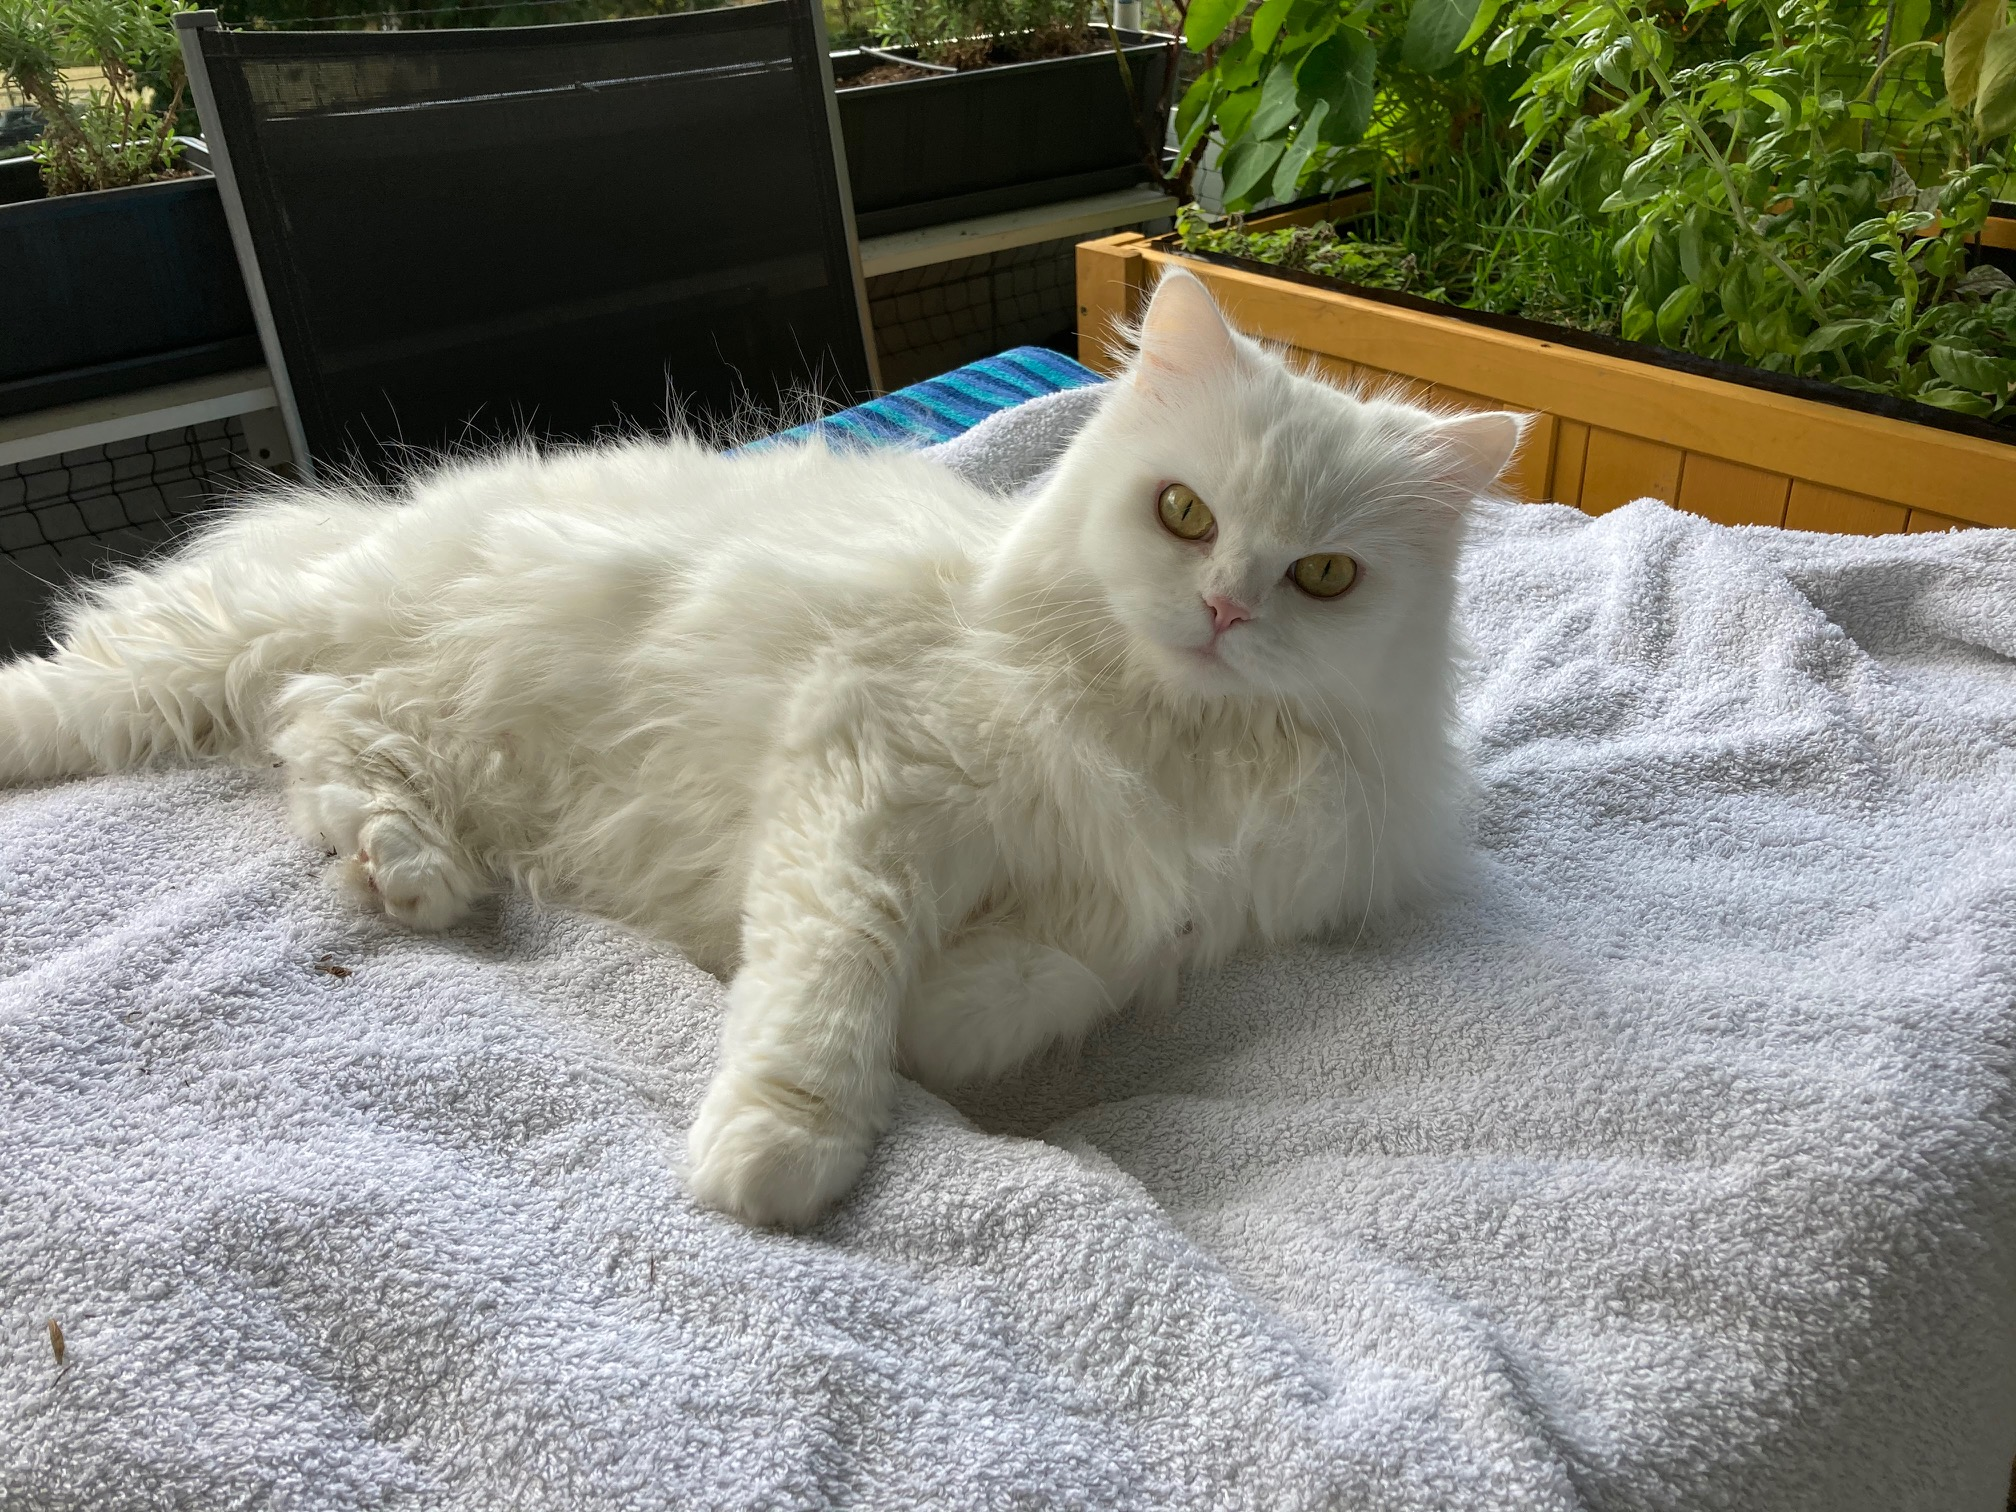
\includegraphics[width=\textwidth]{./Bilder/Katze1}
\caption{Miezekatze}\label{fig:miezekatze}
\end{figure}

\prettyref{fig:miezekatze}

\prettyref{sec:einleitung}

\begin{figure}[h]
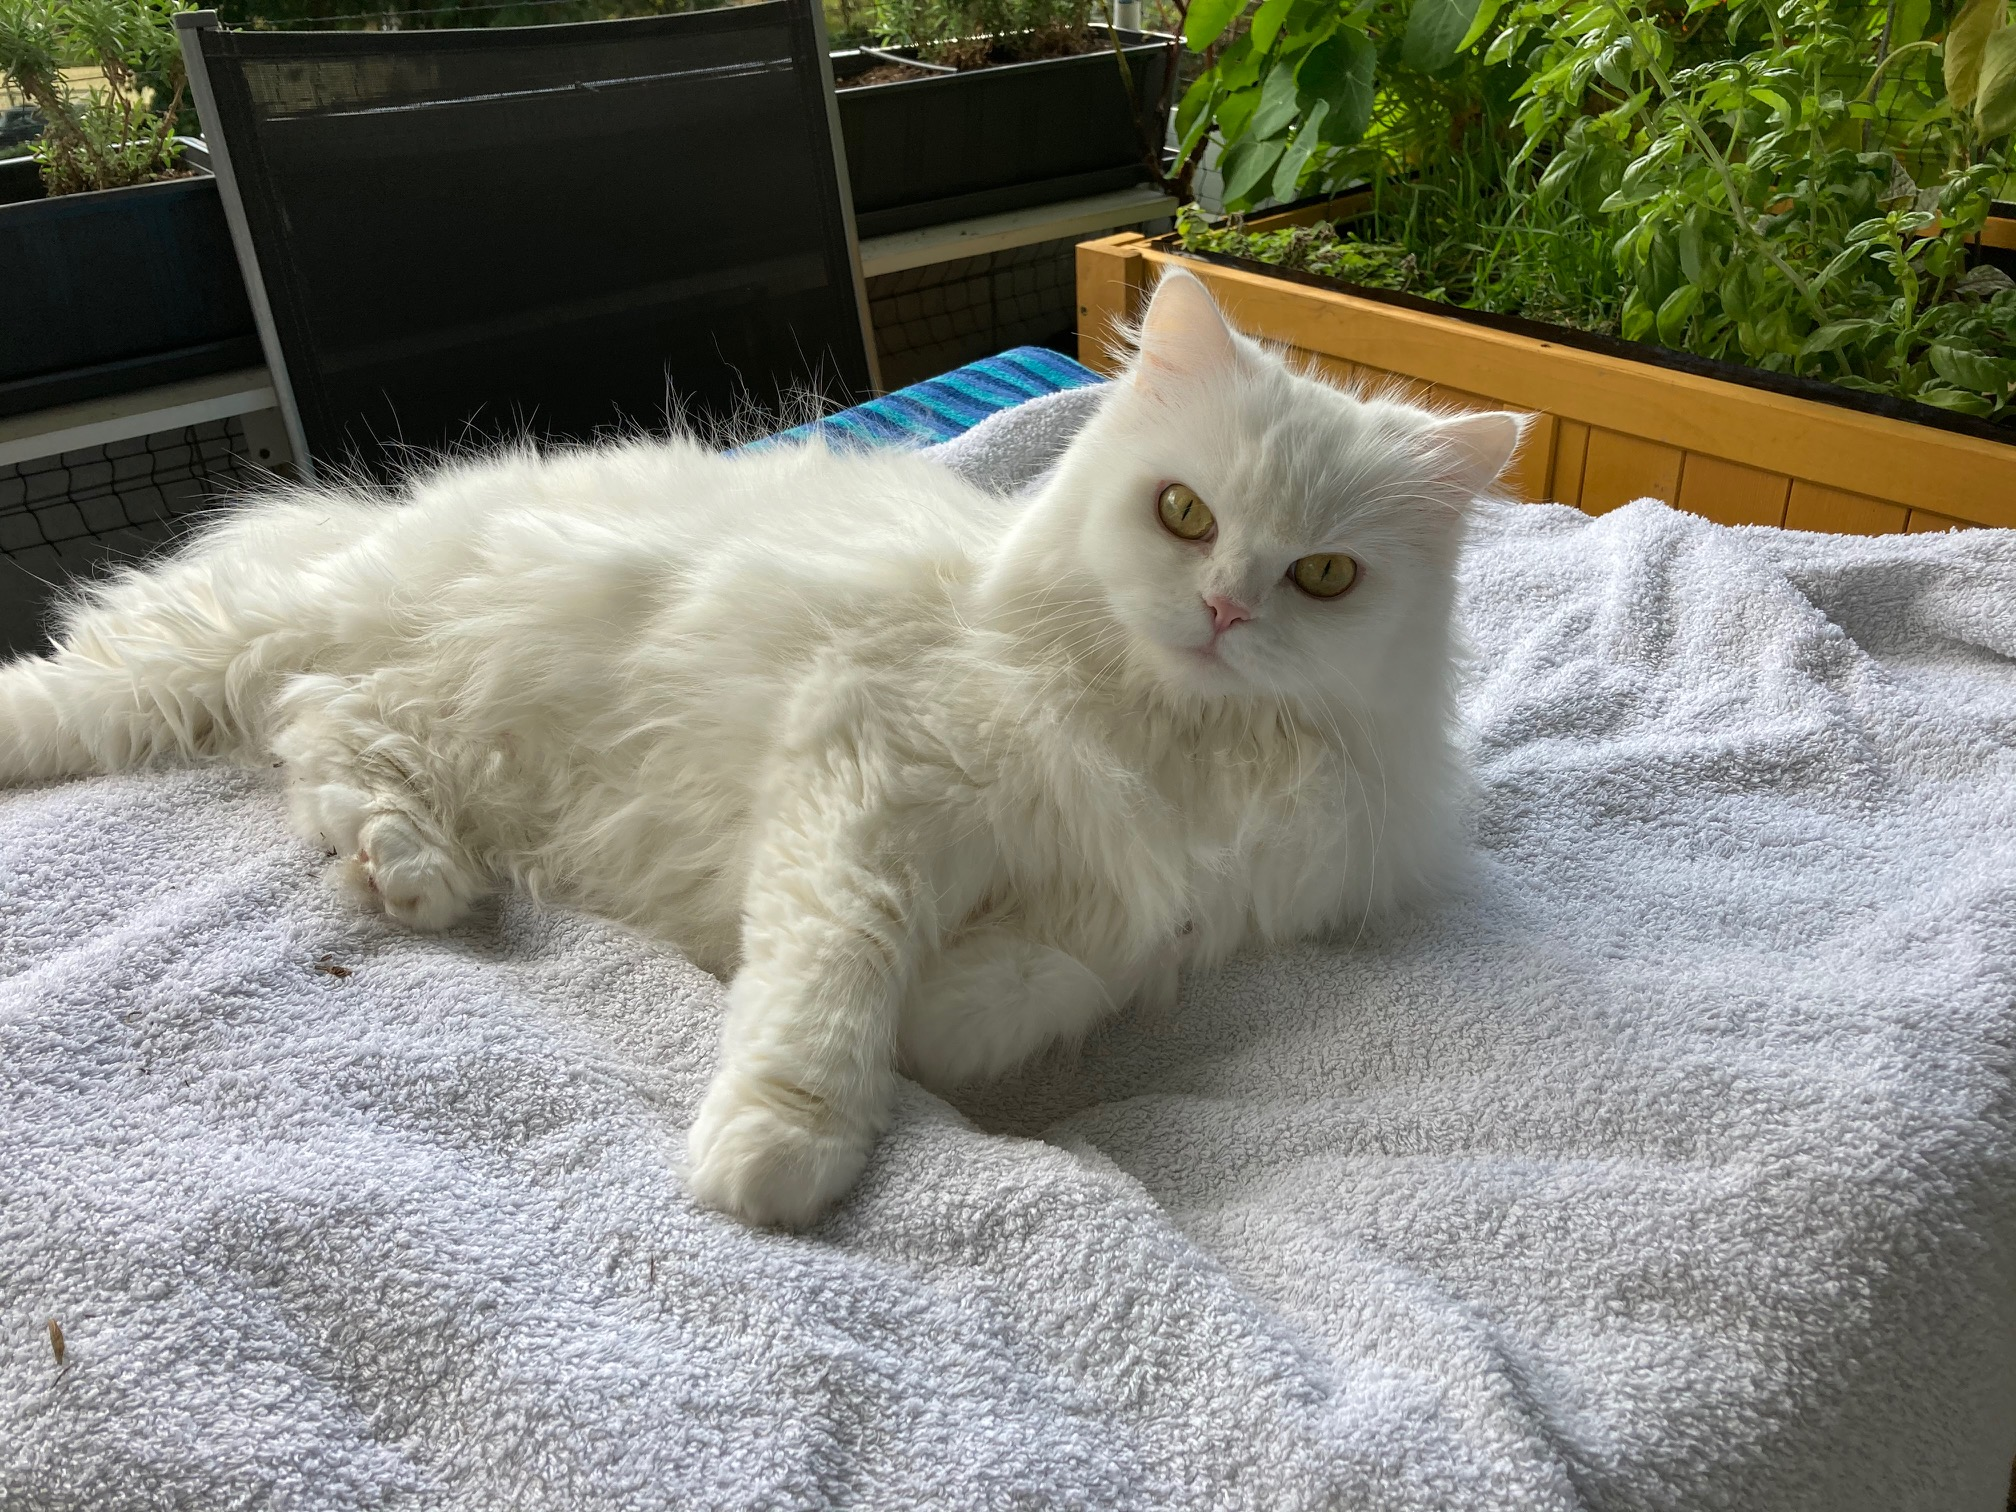
\includegraphics[width=\textwidth]{./Bilder/Katze1}
\caption{Miezekatze}\label{fig:miezekatze2}
\end{figure}

\prettyref{ssec:literatur}

\section{Fazit}\label{sec:fazit}

\blindtext


Abbildung \vref{fig:miezekatze}

\vpageref{fig:miezekatze}

\begin{figure}[h]
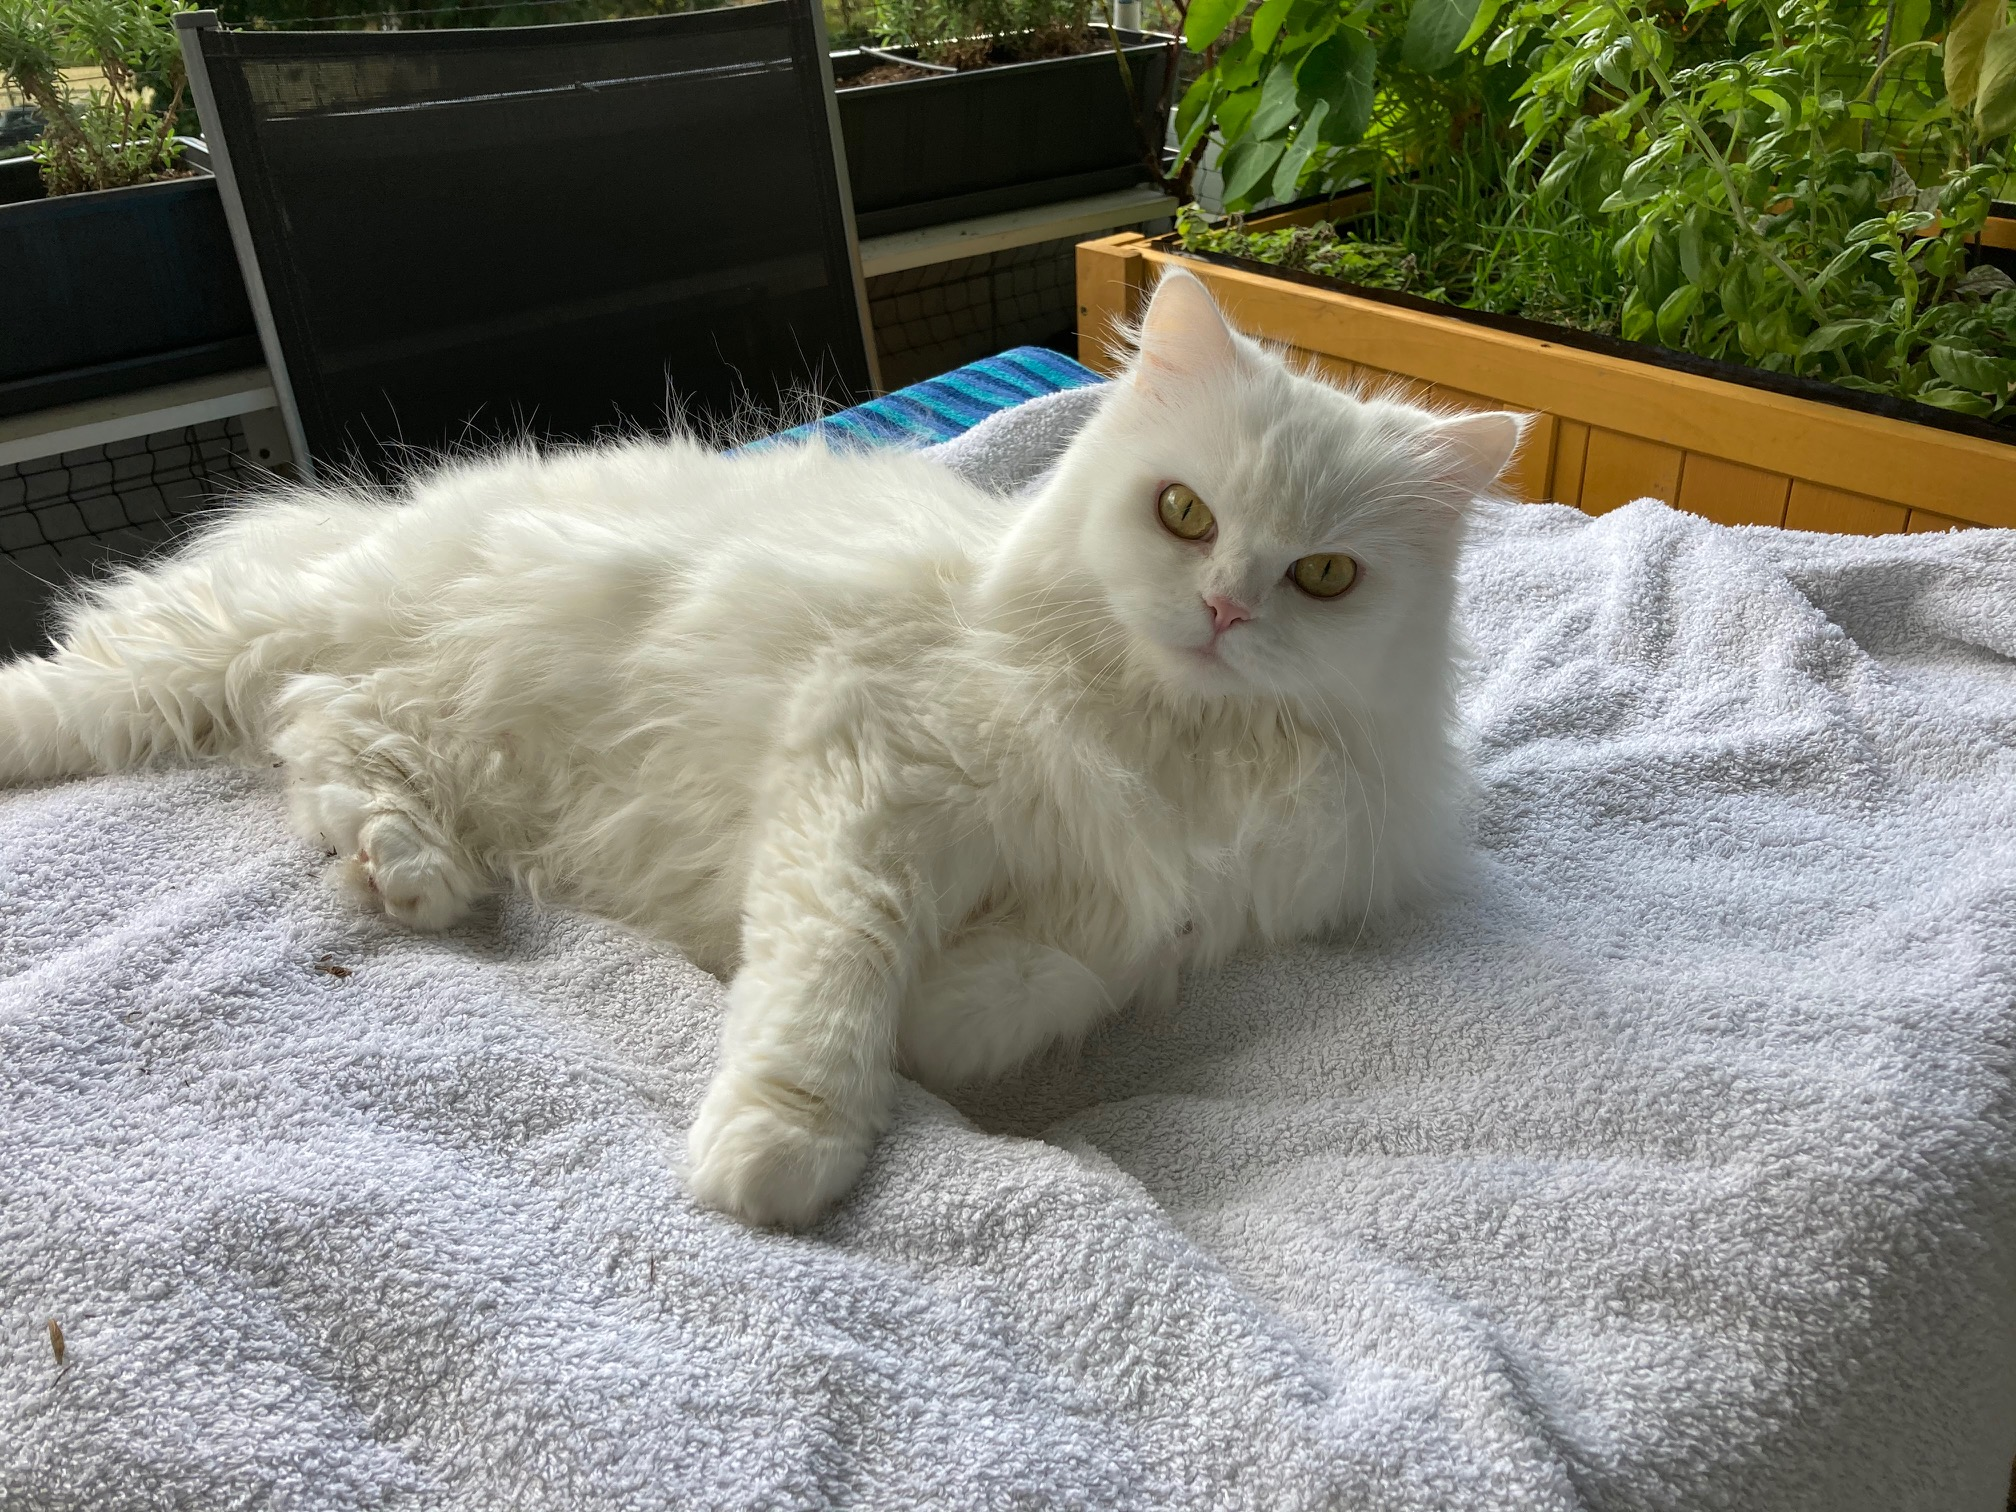
\includegraphics[width=\textwidth]{./Bilder/Katze1}
\caption{Miezekatze}\label{fig:miezekatze3}
\end{figure}

Siehe die Abbildungen \vrefrange{fig:miezekatze}{fig:miezekatze3}

\end{document}